\documentclass[11pt,a4paper]{article}

% --- PACKAGES ---
\usepackage[utf8]{inputenc}
\usepackage[T1]{fontenc}
\usepackage[english]{babel}
\usepackage[margin=2.5cm]{geometry}
\usepackage{helvet}
\renewcommand{\familydefault}{\sfdefault}
\usepackage{microtype}
\usepackage{xcolor}
\usepackage{titlesec}
\usepackage{hyperref}
\usepackage{booktabs}
\usepackage{tabularx}
\usepackage{array}
\usepackage{enumitem}
\usepackage{fancyhdr}
\usepackage{graphicx}
\usepackage{float}
\usepackage{amsmath}
% --- COLOR PALETTE ---
\definecolor{navyblue}{RGB}{20, 45, 85}
\definecolor{tealblue}{RGB}{30, 115, 140}
\definecolor{lightgrey}{RGB}{245, 247, 250}
\definecolor{darkgrey}{RGB}{60, 60, 60}

% --- SETUP HYPERREF ---
\hypersetup{
    colorlinks=true,
    linkcolor=navyblue,
    urlcolor=tealblue,
    pdftitle={Documentazione Progetto AI Maintenance - Business \& Project Management},
    pdfauthor={Gruppo di Progetto}
}

% --- SETUP HEADERS & FOOTERS ---
\pagestyle{fancy}
\fancyhf{}
\rfoot{\small Pagina \thepage}
\renewcommand{\headrulewidth}{0.4pt}
\renewcommand{\footrulewidth}{0.4pt}

% --- SECTION STYLING ---
\titleformat{\section}
  {\color{navyblue}\normalfont\large\bfseries}
  {\thesection}{1em}{}[\titlerule]
\titleformat{\subsection}
  {\color{tealblue}\normalfont\bfseries}
  {\thesubsection}{1em}{}

% --- DOCUMENT BEGIN ---
\begin{document}

% --- TITLE PAGE ---
\begin{titlepage}
    \centering
    
    \begin{center}
        
\includegraphics[width=8cm]{logounipi.png}
    \end{center}
    
    \vspace{0.5cm}
    {\huge \color{tealblue} UNIVERSITÀ DI PISA}\\[0.5cm]
    {\Large \color{navyblue} Dipartimento di ingegneria dell'informazione}\\[0.8cm]
    {\large \color{navyblue} Master's degree in Artificial Intelligence and data engineering}\\[1.5cm]

    {\LARGE \bfseries \color{tealblue} Smart maintenance for automotive businesses}\\[2cm]
    
    \vspace{1.5cm}
    \rule{\linewidth}{0.8pt}
    \vspace{2.5cm}
    
    \begin{minipage}{0.48\textwidth}
        \begin{flushleft} \large
            \textbf{Course:} Business and Project Management\\
            \textbf{Matter:} AI-Driven Business Venture\\
        \end{flushleft}
    \end{minipage}
    \begin{minipage}{0.48\textwidth}
        \begin{flushright} \large
            \textbf{Authors:} Marco Lari, Tommaso Pellegrini\\
            \textbf{Accademic year:} 2025/2026
        \end{flushright}
    \end{minipage}
    \vspace{0.5cm}

    \begin{center} Gitub Repository: \url{https://github.com/marcolari06-maker/BPM-project} \end{center}

    \newpage
    
    \vfill
    \thispagestyle{empty}
    \begin{abstract}
        \noindent In this short paper we present how we intend to organize an AI driven startup in the automotive sector, defining the problem we mean to address and the solutions provided. Furthermore we provide a competitor analysis, a business model canvas, a market estimation and a negative backstacking; evaluating the quality of our own project model.
    \end{abstract}
\end{titlepage}

\tableofcontents
\newpage

% --- SECTION 1: INTRODUCTION AND PROBLEM STATEMENT ---
\section{Introduction to the Problem}
\subsection{Problem and drivers}
\noindent The problem addressed in this paper refers to the inefficiencies and consequent high costs of vehicle maintenance in automotive companies,
such as transportation, logistic and rental businesses.

\subsection*{Problems}
\begin{itemize}
    \item High maintenance costs; costs rose by 8.6\% year over year in 2025, reaching an industry average of 0.215\$ per mile for commercial vehicles in USA. (ATRI report)
    \item Downtime and overhead of maintenance work; the average mileage traveled between brakdowns fell to ~36.500 from ~38.500, indicating that the matter is also worsening over time. (ATRI report)
    \item Parts reperability issues; the rising tariffs on importation and the supply chain directly impact the availability of spare parts. (ATRI report)
\end{itemize}

\subsection*{Drivers}
\begin{itemize}
    \item Unexpected failures of critical components (engine, battery pack, transmission). Companies can't predict failures and are forced to wait for them to happen before taking action.
    \item Unnecessary repairs or replacements to maintain security standard due to lack of predictive maintenance, which leads to periodic schedules or over-maintenance.
\end{itemize}
\subsection{Solution and innovations}
\noindent Given the above problems and drivers, we aim to provide a solution based on a machine learning model that enables to treat such matters with statistical evidence, such that overhead is reduced due to prediction of failures and costs are reduced with less unnecessary maintenance work.
\noindent A machine learning approach is suitable for this kind of problem because unlike fixed rules, heuristic or threshold based approaches, it can learn patterns from data to adapt to situations without the need to make rules for every possible scenario.
\noindent Furthermore it makes the system much more adaptive and scalable, since it can be continuously improved with the collected data, and the data income comes with the normal operation of the vechicles.
\newline\newline
\noindent This kind of approach is innovative in small automotive companies, since is usually adopted as an internal solution by
larger automotive companies, such as OEMs and Tier 1 suppliers. Instead we aim to provide a B2B service that can be adopted by 
smaller realities, such as logistic companies, rental companies and small fleet owners.
\begin{itemize}
    \item Small companies don't have the resources to develop such a system internally.
    \item Previous solutions are heavy on the budget and could be threatening for a upcoming business.
\end{itemize}
Instead in the proposed solution:
\begin{itemize}
    \item The system is provided as a service, with a subscription model, such that the company can pay for the service without having to develop it internally.
    \item The system is designed to be lightweight and easy to integrate with existing systems, such that it can be adopted without major changes to the existing infrastructure.
    \item Even with the cost of the service the overall cost of maintenance is expected to be lower than the current cost, due to the reduction of downtime and unnecessary maintenance work.
\end{itemize}
\subsection{Assumptions}
\begin{itemize} 
    \item Companies agree to install sensors, or already have them and share data with the service provider.
    \item Operational costs of the service are lower than the costs of maintenance even for a small number of vehicles, remaining in line with the target of small companies.
    \item Fleet managers hold sufficient operational budget authority to adopt a new SaaS tool without requiring lengthy corporate procurement approval — relevant because our target includes small-to-mid fleets (30-200 vehicles).
    \item Enough data is available to train the machine learning model before the service is launched, using customer data only for prediction and future improving of the model. 
    \item In its current configuration, the system does not fall under the high-risk AI applications defined by the EU AI Act, as it does not directly control vehicle operation or safety-critical functions. However, the regulatory framework is evolving, and future amendments or national implementations could introduce additional compliance requirements. This uncertainty is treated as a monitored strategic risk (see Section 6.2.7).
\end{itemize} 

% --- SECTION 2: COMPETITORS AND POSITIONING ---
\section{Competitors and Positioning}
\subsection{Patent-based technology screening}

To complement the market review, we conducted a preliminary patent search on Google Patents to assess technological maturity and potential entry barriers in AI-enabled predictive maintenance for commercial fleets. The search combined terms related to predictive maintenance, machine learning, commercial vehicles and fleets, telematics, OBD data and vehicle health. The initial broad search returned documents related to industrial equipment and infrastructure monitoring, so it was refined by adding fleet-specific terms and excluding unrelated domains.
The final results indicate that predictive maintenance based on vehicle sensors, OBD/telematics data and automated analysis is an established technological field. The selected documents include maintenance alert systems, ML-based health assessment, predictive maintenance and approaches designed to operate with limited data. The analysis is intended as a source of competitive and technological intelligence and does not constitute a legal freedom-to-operate assessment.

\renewcommand{\arraystretch}{1.5}
\begin{table}[ht]
\centering
\caption{Patent documents and their main relevance}
\label{tab:patents}
\small
\begin{tabularx}{\linewidth}{p{4cm} X}
\toprule
\textbf{Patent document} &
\textbf{Main relevance} \\
\midrule

US20190066407A1 &
Real-time OBD and sensor-data analysis, fleet-level maintenance alerts, breakdown-pattern analysis and maintenance-cost estimation \\

US12093901B2 &
Telematics-based vehicle-component health assessment using feature extraction, clustering and classification \\

US20230315082A1 &
Predictive maintenance of road-vehicle components \\

EP4379486A1 &
Resource-efficient predictive maintenance for fleets using selected sensors, a digital twin and incremental learning \\

\bottomrule
\end{tabularx}
\end{table}

\noindent The patent screening confirms that the use of AI, telematics and OBD data for predictive maintenance is not novel by itself. Therefore, the proposed venture should differentiate primarily through a lightweight, hardware-agnostic SaaS model for small and medium-sized multi-brand fleets, reduced integration effort and interpretable, prioritized maintenance alerts.

\subsection{Competitive landscape mapping}
\noindent We identify three distinct competitive tiers relevant to a predictive maintenance venture targeting small-to-mid commercial fleets.

\begin{enumerate}
    \item \textbf{Direct Competitors:} Companies offering AI-driven telematics solutions for predictive maintenance, such as:
          \begin{itemize}
            \item \textbf{Carly enterprise:} An affirmed company in the automotive telematics space. Provides predictive maintenance as well as cost calculation, all made for fleets.
            \item \textbf{Steer AI:} A startup that provides predictive maintenance for fleets, with a focus on electric vehicles.
          \end{itemize}
    \item \textbf{Incumbent / OEM:} Established automotive manufacturers and Tier 1 suppliers that offer proprietary predictive maintenance solutions, such as:
            \begin{itemize}
                \item \textbf{Bosch Predictive diagnostics:} a proprietary software solution that continuously monitors component and system health using onboard and cloud data, aimed at preventing breakdowns before they occur
                \item Similar proprietary offerings exist from other Tier-1 suppliers and OEMs.
            \end{itemize}
    \item \textbf{Non AI Substitute Solutions:} Traditional maintenance methods, including:
            \begin{itemize}
                \item Fixed-interval preventive maintenance, still used by the large majority of small and mid-sized fleets. 35\% higher costs and 40\% more breakdowns annually compared to fleets on optimized programs.
                \item Manual visual inspection, costing an estimated \$100-\$300 per vehicle per inspection cycle  and administrative overhead 
                \item Reactive maintenance (repair only after failure),  the most expensive approach; it can cost 3 to 9 times more than the same service performed proactively
            \end{itemize}
\end{enumerate}



\subsection{Assessing Competitors}

The competitors are evaluated according to their value proposition, target
customers, technological scope, integration model and potential limitations.

\subsubsection{Carly Enterprise: Value Proposition, Strengths and Weaknesses}

Carly Enterprise's main value proposition is to make vehicle diagnostics and
maintenance-related information accessible to professional users through a
mobile application, dashboard or API. The platform aims to transform technical
vehicle data into actionable information, such as fault severity, probable root
cause, repair priority and estimated cost.

However, Carly Enterprise also presents potential weaknesses from the
perspective of the target market considered in this project.

\subsubsection{SteerAI: Value Proposition, Strengths and Weaknesses}

SteerAI's value proposition is based on the integration of artificial
intelligence into multiple automotive processes. In the fleet context, the
platform aims to combine vehicle health monitoring, predictive maintenance and
operational workflows in a unified environment.

The main limitation of this approach is the breadth of the platform.
\subsection{Competitor Comparison}

The table below summarizes the main differences between the selected competitors and the proposed venture.

\begin{table}[ht]
\centering
\caption{Comparison of competitors and the proposed venture}
\label{tab:competitor-comparison}
\small
\begin{tabularx}{\linewidth}{p{2.2cm} p{1.8cm} X X X}
\toprule
\textbf{Competitor} &
\textbf{Type} &
\textbf{Main value proposition} &
\textbf{Main strength} &
\textbf{Potential weakness} \\
\midrule

Carly Enterprise &
Direct AI competitor &
Vehicle diagnostics, fault prioritization and predictive maintenance &
Large diagnostic-data base and API/mobile access &
May focus primarily on diagnostic codes and may offer more functionality than small fleets require \\

SteerAI &
Direct AI competitor &
AI platform for diagnostics, fleet operations and automotive workflows &
Broad integration across automotive activities &
Potential complexity and limited publicly available evidence on predictive performance \\

Bosch Predictive Diagnostics &
OEM/Tier-1 incumbent &
Continuous monitoring of vehicle and component health &
Technical expertise and OEM relationships &
Possible ecosystem dependence and lower accessibility for independent fleets \\

Fixed-interval maintenance &
Non-AI substitute &
Simple and familiar scheduled maintenance &
Low technological complexity &
Does not adapt to the actual condition of individual vehicles \\

Reactive maintenance &
Non-AI substitute &
Repair only when a failure occurs &
No investment in predictive systems &
High exposure to downtime, emergency repair and replacement costs \\

Proposed venture &
AI-driven SaaS &
Accessible predictive maintenance for small and medium-sized multi-brand fleets &
Focused product, lightweight integration and hardware-agnostic positioning &
No proprietary large-scale dataset and predictive performance still to be validated \\

\bottomrule
\end{tabularx}
\end{table}

\subsection{Strategic Positioning}

\noindent The proposed venture should not position itself as more accurate than Carly
Enterprise, SteerAI or Bosch before obtaining evidence from a real fleet
pilot. These competitors have access to larger datasets, established
partnerships or broader commercial resources.\newline

\noindent Instead, the proposed differentiation is based on two strategic dimensions.
First, the service is designed specifically for small and medium-sized
multi-brand fleets that may not have the resources to implement a complex
enterprise platform. Second, the system is intended to be lightweight and
hardware-agnostic, allowing integration with existing OBD or telematics
infrastructure wherever possible.\newline

\noindent The venture therefore adopts a focused differentiation strategy rather than a
cost-leadership strategy. Its competitive promise is not to offer the most
complete automotive platform, but to make predictive maintenance easier to
adopt and economically accessible for smaller operators.\newline

\noindent This positioning must be validated through interviews and pilot projects. The
venture can be considered competitively promising only if fleet managers confirm
that the main obstacles of existing solutions are excessive complexity,
integration costs, lack of multi-brand compatibility or insufficient
affordability.\newline

\subsection{Validating competitiveness}
\noindent To demonstrate realistic competitive viability, we provide three arguments:
a quantitative cost-benefit comparison, an explanation of how we compensate for
data-scale disadvantages, and an empirical validation plan. 

\subsection*{Cost-benefit comparison}
\noindent Using ATRI 2026 industry benchmarks, repair and maintenance costs average 
\$0.215 per mile, approximately \$17,200 per vehicle per year at 80,000 miles . 
Unplanned breakdowns occur on average every 36,891 miles, with reactive repairs 
cost 3-9 times more than proactive service. A subscription priced at 
EUR 8--15/vehicle/month (\$108-\$192/year) would be economically viable even with 
conservative savings of 5-10\% on R\&M and 10-20\% on downtime, yielding a net 
benefit of approximately \$770-\$2,500 per vehicle per year 
(5-15 times return on subscription).

\subsection*{Compensating for data-scale disadvantage}
\noindent Despite lacking the proprietary data volume of Carly, SteerAI, or Bosch, we mitigate this through: (i) pretraining on open predictive-maintenance datasets (e.g. NASA) before fine-tuning on real fleet data; (ii) hardware-agnostic, multi-brand integration that serves mixed fleets underserved by OEM-locked solutions; (iii) emphasis on interpretable, actionable warnings over black-box accuracy; and (iv) partnerships with telematics providers or fleet associations.

\subsection*{Empirical validation plan}
\noindent Competitiveness claims will be tested through: 
\begin{enumerate}
    \item 15-30 customer discovery interviews to confirm that existing solutions are too complex, expensive, or brand-restricted for small fleets (success:  > 60\% confirm at least one obstacle); 
    \item a 3-6 month pilot with 50-100 vehicles to measure actual reduction in breakdowns and R\&M costs (success: statistically significant improvement, p < 0.1); 
    \item optional A/B comparison between predictive and fixed-schedule maintenance on vehicle subsets. Until validated, competitiveness remains a hypothesis supported by economic plausibility and strategic differentiation, not an established fact.

\end{enumerate}

% --- SECTION : Business model canvas ---
\section{Business model canvas}
\begin{center}
        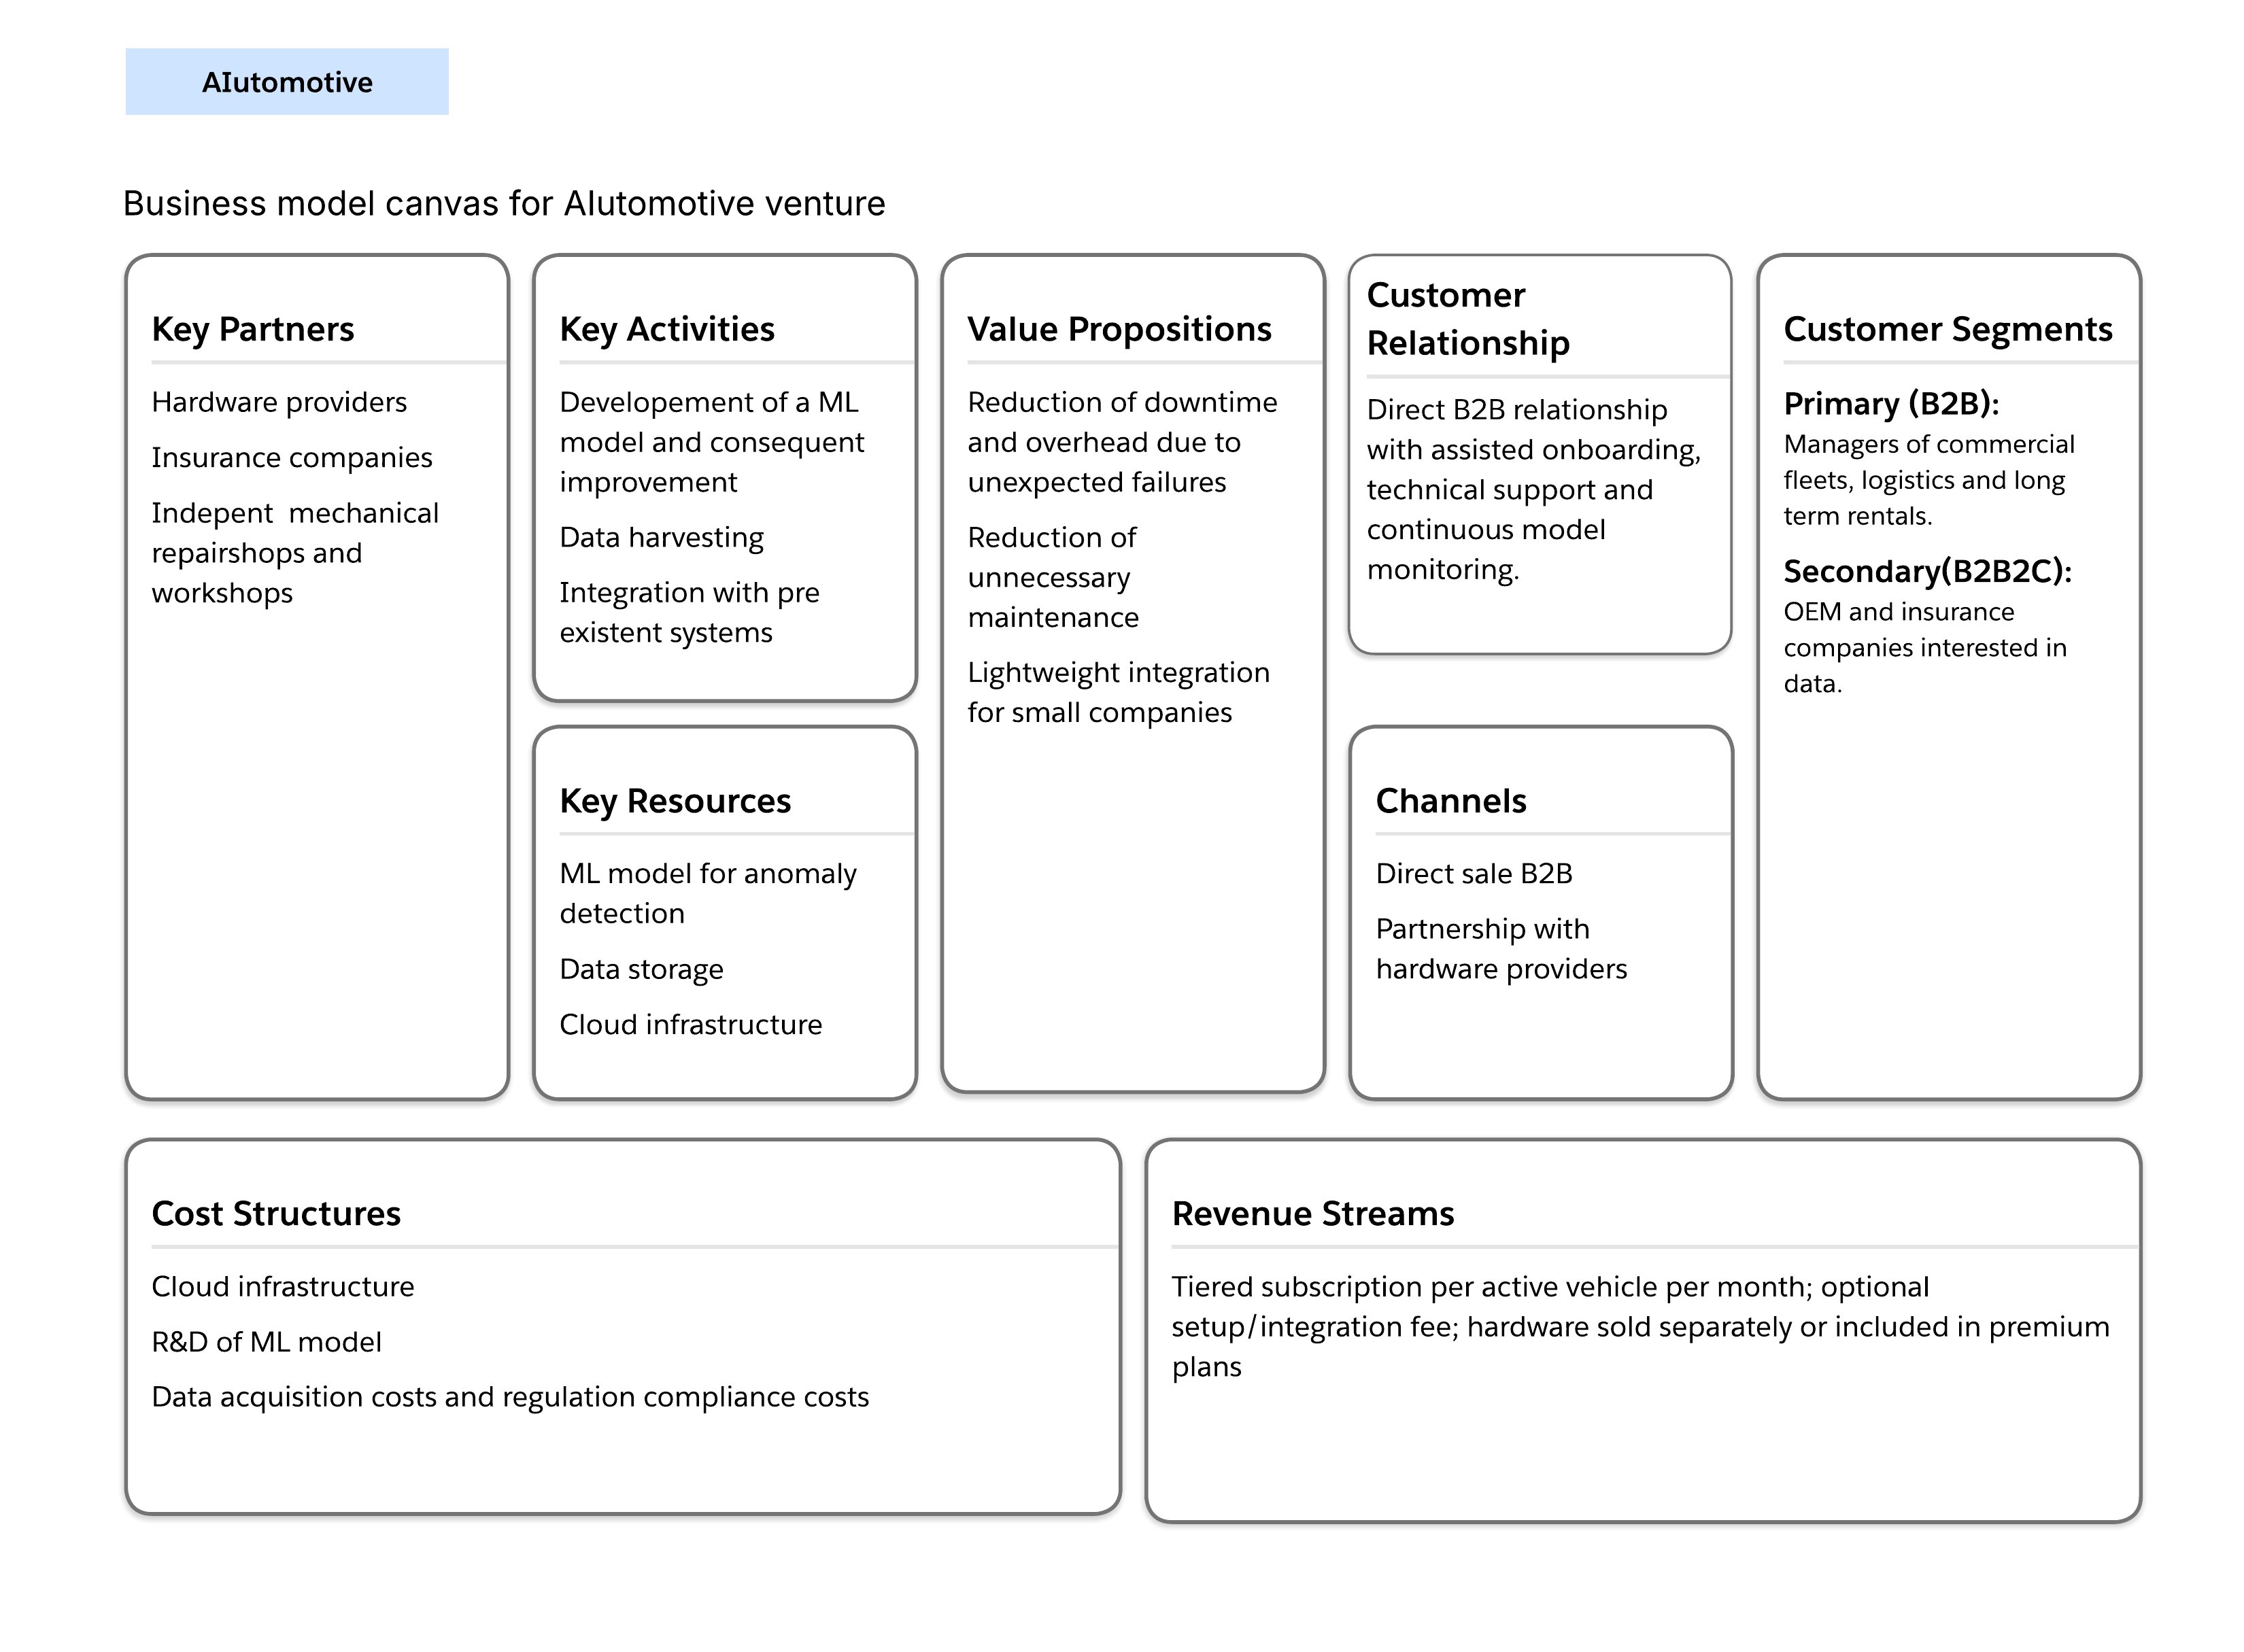
\includegraphics[width=\linewidth]{BMC.png}
\end{center}

\paragraph{Customer segments.}
The primary customer segment consists of managers of commercial fleets, logistics companies and long-term rental businesses. These organizations operate multiple vehicles and are exposed to maintenance costs, unexpected breakdowns and vehicle downtime. The initial target includes small-to-medium-sized companies that may not have the financial or technical resources to develop an internal predictive-maintenance system. A secondary customer segment includes original equipment manufacturers (OEMs) and insurance companies interested in using vehicle-health and maintenance data for operational, analytical or risk-management purposes. The distinction between primary and secondary customers is important because fleet operators are expected to be the initial paying customers, whereas OEMs and insurers may become later-stage customers.

\paragraph{Value propositions.}
The main value proposition is an AI-driven service that uses vehicle data to identify potential anomalies and support more efficient maintenance decisions. The solution aims to reduce downtime and operational overhead caused by unexpected failures. It can also help companies to move from purely scheudled or reactive maintenance toward a more condition-based approach. A further value proposition is lightweight integration: the service is designed to be accessible to smaller companies and to connect with existing hardware and data sources rather than requiring a completely new infrastructure. The system should therefore provide prioritized and understandable alerts instead of only exposing raw diagnostic data.

\paragraph{Channels.}
The main distribution channel is direct B2B sales to fleet managers and other decision-makers within logistics, rental and commercial-transport companies. Direct sales are appropriate during the initial phase. Additional channels may be developed through partnerships with hardware and telematics providers to facilitate access to vehicle data. In a later stage, partnerships with insurance companies, OEMs and other automotive-service providers could support indirect distribution and increase market reach.

\paragraph{Customer relationships.}
The venture will establish a direct B2B relationship with its customers. During the onboarding phase, this relationship will include assisted integration, configuration of data sources and training for fleet and maintenance managers. Continuous technical support will be required because the service depends on data quality, changes in vehicle fleets and the interpretation of maintenance alerts. In addition, the machine-learning models will require continuous monitoring and periodic improvement. As the platform becomes more standardized, part of the onboarding and support process may be automated, while larger customers may continue to receive dedicated technical assistance.

\paragraph{Key activities.}
The main activities include the development and continuous improvement of the machine-learning model, data harvesting and processing, and integration with pre-existing vehicle. Data harvesting involves collecting vehicle measurements, and maintenance events from the available hardwar. The venture must also validate the quality of the data, monitor model performance and translate predictions into useful maintenance recommendations. Commercial activities, such as customer discovery and partnership development, are also necessary to validate the business model and support customer acquisition.

\paragraph{Key resources.}
The main technological resource is the machine-learning model. This is supported by data-storage systems and cloud infrastructure for ingestion, processing and monitoring. Other relevant resources include the expertise of the technical team, maintenance data, software integrations and relationships established with pilot customers and partners. The quality and availability of these resources directly affect the reliability and scalability of the proposed service.

\paragraph{Key partners.}
The main partners are hardware and telematics providers, which supply the sensors or data interfaces required by the service. Independent mechanical repair shops and workshops are also important because they can provide operational knowledge, validate alerts and support the execution of recommended maintenance actions. Insurance companies may become partners by using vehicle-health information for risk assessment or by supporting preventive-maintenance programs. These partnerships can reduce customer-acquisition barriers, improve access to data and strengthen the credibility of the venture.

\paragraph{Revenue streams.}
The primary revenue stream is a tiered subscription charged for each active vehicle per month. A per-vehicle pricing model aligns the cost of the service with the size of the customer fleet and allows the venture to generate recurring revenue. Different subscription tiers may reflect differences in data volume, level of technical support, number of integrations and availability of advanced analytics. Additional revenue may come from a one-time setup or integration fee for more complex deployments. Hardware can either be sold separately or included in premium plans, depending on whether customers already possess compatible equipment.

\paragraph{Cost structure.}
The main cost drivers are cloud infrastructure, research and development of the machine-learning model, data-acquisition costs and regulatory-compliance costs. Although the cost per additional vehicle may decrease as the platform scales, initial investments in software development, integrations and model validation are expected to be significant.
\\
\\ Overall, the Business Model Canvas highlights the relationship between the operational problem faced by commercial fleets and the economic logic of the proposed solution. The venture creates value by transforming vehicle data into actionable maintenance information, delivers this value through direct B2B relationships and technical partnerships, and captures value primarily through recurring subscriptions. However, the feasibility of the model depends on several assumptions, including access to reliable data, acceptable integration costs, customer willingness to pay and the ability of the machine-learning system to generate measurable reductions in downtime and unnecessary maintenance. The following section describes the machine-learning pipeline that supports this business model.


\subsection{AI Assets and Economic Logic}

The AI component creates value through the relationship between data, models and computational infrastructure. More reliable vehicle data can improve anomaly detection; better predictions can increase customer value; higher customer adoption can generate more data for further model improvement. This creates a reinforcing learning mechanism, although it should not be assumed automatically.

The business model is scalable if the platform can serve additional vehicles without a proportional increase in personnel, integration effort or infrastructure costs. A standardised software architecture, reusable integrations and automated model monitoring are therefore important. However, hardware installation, customer-specific configurations and fragmented vehicle data may limit scalability.

The venture should measure unit economics through indicators such as customer acquisition cost, monthly recurring revenue per vehicle, gross margin per vehicle, churn rate and customer lifetime value. Feasibility improves when the lifetime value of a customer clearly exceeds acquisition and onboarding costs, while the gross margin remains sufficient to finance model development and support.

\subsection{Machine Learning Pipeline}

\subsubsection{Overview}
\noindent The predictive maintenance system relies on two distinct pipelines: a \textbf{training pipeline}, executed offline to build and validate the model, and an \textbf{inference pipeline}, executed in production to generate real-time predictions on incoming telemetry data. Separating these two pipelines is essential both for engineering clarity and to prevent inconsistencies between how features are computed during training and during deployment.

\begin{figure}[htbp]
    \centering
    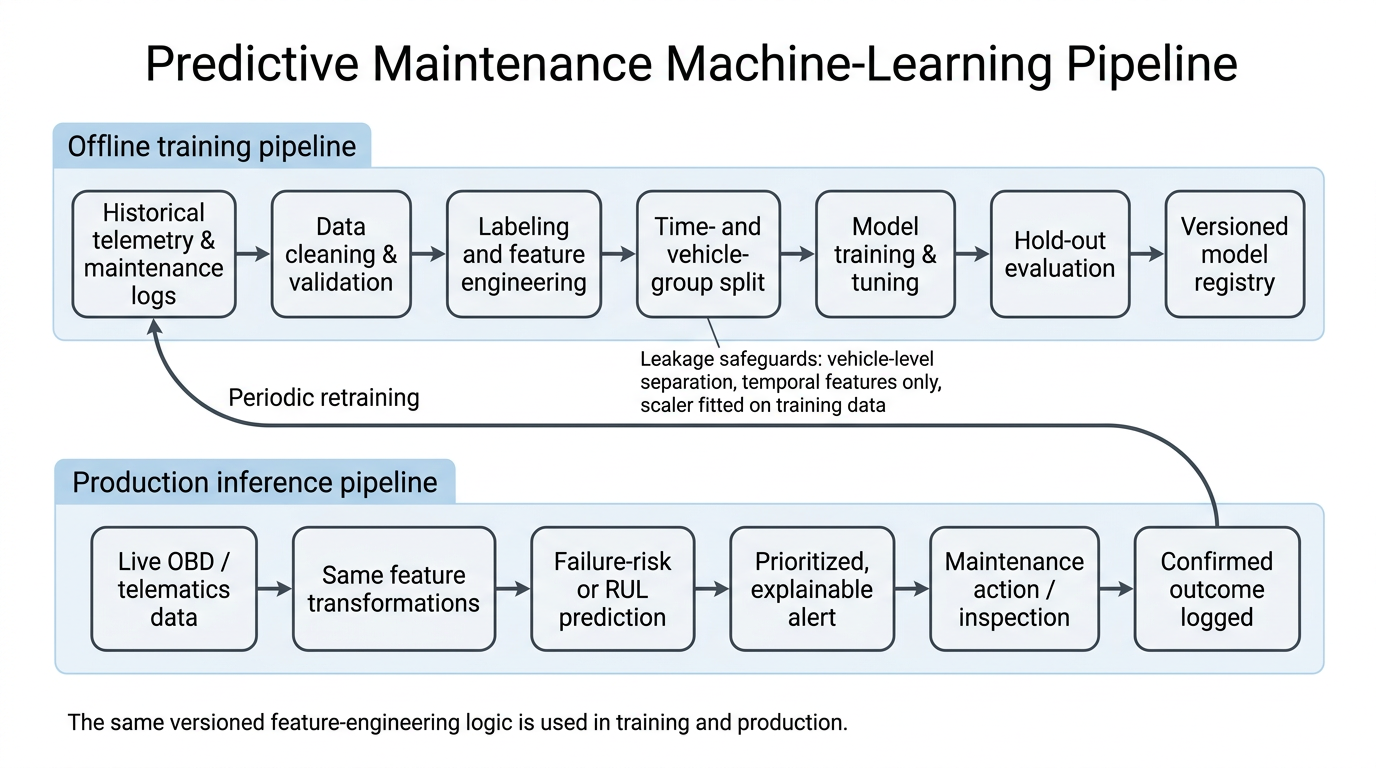
\includegraphics[width=0.75\textwidth]{pipeline.png}
    \caption{Business Model Canvas for the AI-driven predictive-maintenance venture.}
    \label{fig:bmc_canvas}
\end{figure}

\subsubsection{Training Pipeline}

\begin{enumerate}
    \item \textbf{Data Ingestion:} raw telemetry (OBD-II codes, sensor readings such as engine temperature, vibration, battery voltage) and maintenance logs are collected per vehicle, timestamped, and stored in a structured format (vehicle ID, timestamp, sensor readings, maintenance events).
    \item \textbf{Data Cleaning:} removal of duplicate readings, handling of missing sensor values (via forward-fill within a vehicle's own history, never via global imputation that could leak information across vehicles), and outlier filtering based on physically plausible sensor ranges.
    \item \textbf{Labeling:} for each vehicle, a target variable is defined, either as \textit{Remaining Useful Life} (RUL, regression) or as a \textit{binary failure-within-horizon} flag (classification, e.g. "will this component fail within the next 30 days?"). Labels are constructed strictly using each vehicle's own historical failure records.
    \item \textbf{Feature Engineering:} rolling statistics (mean, standard deviation, trend slope) are computed over fixed historical windows (e.g. last 7/30 days) using only past observations relative to each timestamp.
    \item \textbf{Train/Validation/Test Split:} performed with strict temporal and group-based separation (see Section~\ref{sec:leakage} for details).
    \item \textbf{Model Training:} candidate models (gradient boosting for tabular features, or LSTM/Transformer architectures for raw sequential data) are trained on the training set only.
    \item \textbf{Hyperparameter Tuning:} performed via cross-validation restricted to the training set, using time-aware or group-aware folds, never on the held-out test set.
    \item \textbf{Evaluation:} final performance is measured once on the untouched test set, using metrics appropriate to the task (RMSE/MAE for RUL regression; precision, recall and F1 for failure classification, given the expected class imbalance).
\end{enumerate}

\subsubsection{Inference Pipeline}

\begin{enumerate}
    \item \textbf{Real-Time Data Collection:} incoming telemetry from a vehicle is streamed or batched at regular intervals.
    \item \textbf{Feature Computation:} the same feature transformations defined during training (identical rolling windows, identical scaling parameters fitted on the training set) are applied to the incoming data, ensuring train/serve consistency.
    \item \textbf{Prediction:} the trained model outputs either an estimated RUL or a failure probability within the defined horizon.
    \item \textbf{Alert Generation:} predictions are filtered through a decision threshold (calibrated during validation, not on test data) and translated into prioritized, human-readable alerts for the fleet manager.
    \item \textbf{Feedback Loop:} confirmed outcomes (actual failures, false alarms, maintenance actions taken) are logged and periodically fed back into the training pipeline for model retraining, always respecting the same leakage-prevention rules applied to the original training data.
\end{enumerate}

\subsubsection{Data Leakage Prevention}
\label{sec:leakage}

\noindent Data leakage is a critical risk in predictive maintenance settings, where naive splitting strategies can produce artificially high validation performance that does not generalize to real deployment. The following safeguards are applied throughout the pipeline.

\begin{itemize}
    \item \textbf{Group-based splitting (by vehicle):} data from the same vehicle must never appear in both the training and test sets, even at different timestamps. Splitting must be performed at the vehicle level (e.g. 70\% of vehicles for training, 15\% for validation, 15\% for test), not at the observation level. Random row-level splitting would leak vehicle-specific patterns (driving style, component batch, maintenance history) between sets, inflating apparent accuracy.
    \item \textbf{Temporal splitting:} within the training vehicles, features must be computed using only information available up to the prediction timestamp. Rolling windows, cumulative statistics or trend features must never include future observations relative to the point being predicted.
    \item \textbf{No global normalization:} scaling and normalization parameters (mean, standard deviation, min/max) must be fitted exclusively on the training set and then applied unchanged to validation and test sets. Fitting a scaler on the full dataset before splitting is a common and subtle leakage source.
    \item \textbf{Target leakage avoidance:} features that are only recorded at or after the failure event (e.g. a diagnostic code generated as a consequence of the failure itself) must be excluded from the feature set, since they would not be available at prediction time in a real deployment scenario.
    \item \textbf{Cross-validation strategy:} hyperparameter tuning must use group-aware and time-aware cross-validation (e.g. \texttt{GroupKFold} or a rolling-origin time series split), rather than standard k-fold, to preserve the same separation guarantees as the main train/test split.
    \item \textbf{Consistent feature computation at inference time:} any transformation applied to raw data during training (imputation rules, rolling window definitions, encoding of categorical variables) must be implemented identically in the inference pipeline, ideally through a shared, versioned feature-engineering module, to avoid training/serving skew.
\end{itemize}

\noindent These safeguards are particularly relevant given the assumption, introduced in Section~1, that the model may initially rely on open datasets (e.g. NASA Turbofan) before sufficient proprietary fleet data is collected. Since such datasets differ in domain from commercial road vehicles, any transfer learning or fine-tuning step must preserve the same group- and time-based separation logic when the model is later retrained on real customer data, to avoid conflating benchmark validation performance with production-readiness.

\subsection{Critical Assumptions and Interdependencies}

The business model depends on several critical assumptions:
\begin{itemize}
    \item Vehicle data is available, sufficiently accurate and legally usable.
    \item The model can detect relevant anomalies with enough precision to justify customer adoption.
    \item Fleet managers are willing to change from reactive or scheduled maintenance to data-supported decisions.
    \item Integrations with existing systems can be completed without excessive time or cost.
    \item Customers perceive the reduction in downtime and unnecessary maintenance as greater than the subscription and implementation costs.
    \item Hardware providers, repair shops, OEMs and insurers are willing to cooperate under commercially acceptable conditions.
\end{itemize}

\noindent These assumptions are interdependent. For example, model accuracy depends on data quality, while data quality depends on hardware reliability and customer usage. Customer willingness to pay depends on measurable economic benefits, but those benefits can only be demonstrated through successful integration and sufficient operating data. Similarly, scalability depends on standardising deployments, while standardisation may be difficult if vehicles and customer systems differ substantially.

\subsection{Feasibility and Scalability Assessment}

The model is potentially feasible because it addresses a costly and recurring operational problem and generates recurring revenue. Its strongest economic logic is the link between preventive predictions and reduced downtime. However, feasibility should be tested through pilots rather than assumed: initial pilots should compare a customer’s maintenance performance before and after implementation using indicators such as unexpected failures, downtime hours, maintenance expenditure and vehicle utilisation.
\\
Scalability is strongest on the software side. Once the platform and model are operational, adding vehicles can increase recurring revenue without requiring a complete redesign of the service. The main scalability constraints are data heterogeneity, hardware deployment, customer-specific integration and the need to maintain prediction quality across different vehicle fleets.
\\
The venture should therefore follow a staged growth path. It should first focus on a limited group of fleet customers and a defined set of vehicle types. After validating the value proposition and unit economics, it can expand through standardised integrations, hardware partnerships and indirect distribution via OEMs or insurers. This approach reduces execution risk and ensures that growth is based on demonstrated operational and financial performance.
% --- SECTION 4: ADA
\section{Addressable market analysis}
\noindent This section quantifies the economic opportunity for the proposed venture by estimating the Total Addressable Market (TAM), Serviceable Addressable Market (SAM), and Serviceable Obtainable Market (SOM) adopting a bottom-up methodology. We started from the number of potential customer fleets in the United States then multiplied by the expected annual subscription revenue per vehicle, consistently with the customer segment and pricing assumptions defined in Sections 1-3.

\subsection{Data source and scope}
The primary data source for fleet counts is the FMCSA Company Census (dataset az4n-8mr2), which reports active registered motor carriers by fleet size updated on August 2026. According to this registry, there are ~2,230,000 active carriers in the U.S., of which ~700,000 are interstate carriers and ~330,000 hold active common (for-hire) operating authority. Fleet size distribution shows that ~40,000 carriers report 21-100 power units and ~8,000 carriers report 101+ power units.
\\
\\
The analysis focuses on for-hire carriers with 30-200 vehicles, as this segment matches our target. Carriers with fewer than 30 vehicles are excluded because they typically operate with informal maintenance practices and limited telematics adoption. Carriers with more than 200 vehicles are excluded because they often have proprietary solutions from OEMs or Tier-1 suppliers (e.g., Bosch Predictive Diagnostics) or internal data science teams, making them less suitable for our proposal.

\subsection{Total Addressable Market (TAM) Estimation}
To estimate the number of carriers in the 30-200 vehicle range, we apply conservative proportional assumptions to the FMCSA buckets:
\begin{itemize}
    \item 21-100 bucket (~40,000 carriers): We assume 55\% of these carriers fall in the 30-100 range (the remainder are 21-29 vehicles). This yields approximately ~22,000 carriers.
    \item 101+ bucket (~8,000 carriers): We assume 35\% of these carriers fall in the 101-200 range (the remainder are 201+ vehicles, which are enterprise fleets less relevant to our positioning). This yields approximately ~2,800 carriers.
\end{itemize}
Summing these gives a TAM of approximately 24,800 carriers in the U.S. with 30-200 vehicles.
To convert carriers to vehicles, we assume an average fleet size of 65 vehicles (midpoint of the 30-200 range, slightly conservative to account for the right-skewed distribution where more carriers cluster near the lower end). This yields an estimated 1,612,000 vehicles in the TAM segment.
Applying the midpoint subscription price of USD 12.5/vehicle/month, the annual revenue per vehicle is USD 150. Therefore:
\begin{equation}
    \text{TAM} = \underbrace{1{,}612{,}000}_{\text{vehicles}} \times \underbrace{150}_{\text{USD/vehicle/year}} \approx 241.8 \text{ million USD/year}
\end{equation}

\subsection{Serviceable Addressable Market (SAM) Estimation}
Not all TAM carriers are immediately addressable. Based on the assumptions in Section 1.3 and 3.2, we exclude carriers that:
\begin{itemize}
    \item Operate primarily intrastate with no interstate authority (less likely to invest in advanced telematics).
    \item Are not multi-brand (single-brand fleets may prefer OEM-locked solutions like Bosch).
    \item Lack existing telematics or OBD-II data access (our solution assumes sensor data is already available or can be installed with minimal overhead).
\end{itemize}
We estimate that 40\% of the TAM meets these criteria (multi-brand, digital-ready, budget authority for SaaS tools). Therefore:
\begin{equation}
    \text{SAM} = \underbrace{1{,}612{,}000}_{\text{vehicles}} \times \underbrace{0.40}_{\text{proportion}} \approx 645{,}000 \text{ vehicles}
\end{equation}
\begin{equation}
    \text{SAM (USD/year)} = 241.8 \text{ million} \times 0.40 \approx 96.7 \text{ million USD/year}
\end{equation}

\subsection{Serviceable Obtainable Market (SOM) Estimation}
Given the early-stage nature of the venture (no proprietary large-scale dataset, predictive performance still to be validated via pilots as stated in Section 2.5), a realistic market penetration rate by Year 3 is 3\% of the SAM. This is consistent with typical SaaS adoption curves for niche B2B verticals and aligns with the staged growth path described in Section 3.3 (start with a limited group of pilot customers, then expand through standardized integrations).
\begin{equation}
    \text{SOM (vehicles, Year 3)} = 645{,}000 \times 0.03 \approx 19{,}350 \text{ vehicles}
\end{equation}
\begin{equation}
    \text{SOM (USD/year, Year 3)} = 96.7 \text{ million} \times 0.03 \approx 2.9 \text{ million USD/year}
\end{equation}  

\subsection{Investment justification}
The SOM of ~2.9 million USD/year by Year 3 represents a credible revenue base for an early-stage AI venture. Using ATRI benchmarks, repair and maintenance costs average USD 0.215/mile, or approximately USD 17,200/vehicle/year at 80,000 miles. A subscription priced at USD 108-192/vehicle/year would be economically viable even with conservative savings of 5-10\% on R\&M and 10-20\% on downtime, yielding a net benefit of approximately USD 770-2,500/vehicle/year (5-15× return on subscription cost), as assumed in the previous section. 
\\
\\ 
This implies (customer liftime value) LTV » CAC (customer acquisition cost) and sufficient gross margin to fund model development. The market opportunity therefore justifies the initial investment, provided that the planned validation (15–30 interviews and a 3–6 month pilot with 50–100 vehicles) confirms the assumed pain points and cost savings.


\begin{table}[h!]
\centering
\small
\begin{tabularx}{\linewidth}{l r r r X}
\toprule
\textbf{Level} & \textbf{Carriers} & \textbf{Vehicles} & \textbf{Annual Revenue (USD)} & \textbf{Logic} \\
\midrule
TAM & $\sim$24,800 & $\sim$1,612,000 & $\sim$241.8 M &
All U.S. for-hire carriers with 30--200 vehicles; USD 150/vehicle/year \\
SAM & $\sim$9,900 & $\sim$645,000 & $\sim$96.7 M &
40\% of TAM: multi-brand, digital-ready, SaaS budget authority \\
SOM (Y3) & $\sim$300 & $\sim$19,350 & $\sim$2.9 M &
3\% of SAM by Year 3; staged growth via pilots and standardized integrations \\
\bottomrule
\end{tabularx}
\caption{Market sizing summary: TAM, SAM, and SOM.}
\label{tab:market-sizing}
\end{table}


% --- SECTION 5:Personas and validation strategies---
\section{Personas and Validation Strategies}
\noindent This section defines the user personas that will guide market testing and describes the validation strategy for the proposed venture. The analysis still focuses on small-to-mid commercial fleets (30-200 vehicles) in the United States and treats all claims about customer adoption, data availability and economic benefits as hypotheses to be tested.

\subsection{Validation objectives}
\noindent The primary objectives of the market test are to:
\begin{itemize}
    \item Confirm that unplanned downtime and reactive maintenance are perceived as high-priority, costly problems by the target segment.
    \item Validate that existing alternatives (fixed-interval maintenance, OEM solutions, enterprise telematics platforms) are considered too complex, expensive or brand-restricted for small-to-mid fleets.
    \item Assess whether target fleets have or can provide sufficiently reliable OBD or telematics data with acceptable integration effort.
    \item Estimate willingness to pay within the proposed range of USD 8-15 per vehicle per month (approximately USD 96-180 per year).
    \item Obtain early evidence that a pilot deployment can generate measurable improvements in downtime, emergency repairs or total repair-and-maintenance expenditure.
\end{itemize}

\subsection{User Personas}
\indent Two primary personas are defined to guide customer discovery, MVP design and pilot recruitment. Both personas are fictitious but representative of real decision-makers and users in the target segment.
\subsubsection{Persona 1 - Fleet manager}
\noindent \textbf{Name and profile:} Peter Parker, Fleet Manager at a regional logistics company operating 80 commercial vehicles.
\\ \noindent \textbf{Role:} Responsible for fleet availability, maintenance budget, on-time delivery performance and selection of operational tools. Approves or co-approves software expenditures for fleet management and maintenance.
\\ \noindent \textbf{Context:}  Manages a mixed fleet of 30-200 vehicles. Receives data from telematics providers, workshops and drivers, but often plans maintenance using fixed schedules and fragmented spreadsheets or legacy software.
\vspace{0.5cm}
\\\textbf{Goals:}
\begin{itemize}
    \item Minimize unplanned downtime and breakdown-related delivery delays.
    \item Make maintenance costs more predictable and reduce emergency repairs.
    \item Maintain high vehicle utilization without excessive over-maintenance.
    \item Justify technology investments to senior management with clear ROI.
\end{itemize}

\noindent \textbf{Frustrations:}
\begin{itemize}
    \item Unexpected component failures (engine, transmission, battery) that disrupt operations.
    \item High and volatile repair costs, especially for urgent interventions.
    \item Lack of integrated, actionable insights from existing telematics or maintenance tools.
    \item Enterprise platforms perceived as too expensive, complex or tied to specific OEMs.
\end{itemize}
\vspace{0.5cm}
\noindent \textbf{Job-to-be-done:} “When I manage a mixed commercial fleet, I want to identify vehicles likely to fail before a breakdown occurs, so that I can schedule maintenance with minimal disruption and cost.”
\\ \noindent \textbf{Decision power:} Can initiate a pilot or approve a low-cost SaaS subscription independently; larger investments require management or procurement approval. This aligns with the assumption in Section 1.3 that fleet managers in small-to-mid fleets hold sufficient operational budget authority to adopt a new SaaS tool without long corporate procurement processes.

\subsubsection{Persona 2 - Maintenance manager/Workshop manager}
\noindent \textbf{Name and Profile:} Steve Rogers, Maintenance Manager at a rental and logistics fleet with 120 vehicles.
\\ \noindent \textbf{Role:} Plans and coordinates all maintenance activities, manages internal technicians and external workshops, verifies anomalies, records repairs and downtime.
\\ \noindent \textbf{Context:} Handles competing priorities between scheduled maintenance and urgent repairs. Uses OBD data, GPS/telematics platforms, spreadsheets or dedicated fleet-maintenance software.
\vspace{0.5cm}
\\\textbf{Goals:}
\begin{itemize} 
    \item Detect potential failures early enough to schedule interventions proactively.
    \item Reduce the number of emergency repairs and associated overtime costs.
    \item Organize spare parts and workshop workload more efficiently.
    \item Avoid false alarms that waste time and undermine trust in the system.
\end{itemize}
\textbf{Frustrations:}
\begin{itemize}
    \item Alerts that are difficult to interpret or not linked to clear actions.
    \item Fragmented or low-quality data from multiple sources.
    \item Long and costly integration projects with existing systems.
    \item Complex dashboards that do not fit daily operational routines.
\end{itemize}
\vspace{0.5cm}
\noindent \textbf{Job-to-be-done:} “When the system detects a possible component failure, I want an understandable and actionable warning, so that I can inspect or service the right vehicle before it becomes unavailable.\newline
\\
\noindent \textbf{Adoption condition:} Will actively use the system only if alerts are interpretable, prioritized and connected to concrete maintenance actions. This reflects the critical assumption in Section 3.2 that customers must perceive the reduction in downtime and unnecessary maintenance as greater than the subscription and implementation costs .\

\subsection{Key hypotheses to validate}
\noindent The market test focuses on the following hypotheses, which are directly derived from the problem definition, competitive positioning and business model described in Sections 1-3 :
\\
\begin{table}[h!]
\centering
\small
\begin{tabularx}{\linewidth}{l X X}
\toprule
\textbf{ID} & \textbf{Hypothesis} & \textbf{Criticality} \\
\midrule
H1 &
Fleet managers in the target segment experience costly and frequent unplanned downtime and consider it a priority operational problem. &
Validates problem--solution fit. \\

H2 &
Small-to-mid fleets perceive current predictive-maintenance alternatives as too expensive, complex or OEM-locked. &
Validates strategic positioning versus Carly Enterprise, SteerAI and Bosch. \\

H3 &
Target fleets can provide sufficiently reliable OBD or telematics data with acceptable integration effort. &
Validates data availability and hardware-agnostic positioning. \\

H4 &
Maintenance managers consider predictive alerts useful only if they are understandable, prioritized and actionable. &
Validates UX and operational adoption. \\

H5 &
Fleet managers are willing to pay within the proposed range of USD 8--15 per vehicle per month if value is demonstrated. &
Validates revenue model and unit economics. \\

H6 &
A pilot deployment can generate measurable improvements in downtime, emergency repairs or maintenance expenditure. &
Validates economic impact promised in Section~2.5. \\

\bottomrule
\end{tabularx}
\caption{Key hypotheses to be validated through market testing.}
\label{tab:hypotheses}
\end{table}

\subsection{Validation Strategy Methods}
\noindent The validation strategy combines qualitative customer discovery with quantitative pilot evidence, following a staged approach that reduces execution risk before scaling.

\subsubsection{Customer Discovery Interviews}
\noindent We will conduct 15--30 semi-structured interviews with fleet managers and maintenance managers in the target segment. Interviews will explore current maintenance practices with consequent problems, experience with existing tools, data availability and willingness to pay. We state as success criterion that at least 60\% of interviewees confirm at least one major obstacle with current solutions (complexity, cost, OEM lock-in or lack of actionable insights), consistent with hypotheses H1 and H2.

\subsubsection{Survey}
\noindent A short online survey (10--12 questions) will be distributed to a broader sample to quantify the prevalence of the problems identified in interviews. The survey will include Likert-scale items on downtime frequency, maintenance cost volatility, satisfaction with current tools and price sensitivity. Results will triangulate interview findings and refine the definition of the target segment.

\subsubsection{MVP (Minimum Viable Product)}
\noindent The MVP will consist of a cloud-based dashboard that ingests OBD or telematics data from a limited set of vehicle models and provides:
\begin{enumerate}
    \item daily vehicle health scores;
    \item ranked alerts with estimated failure probability and recommended actions;
    \item a simple cost-savings estimator.
\end{enumerate}
\noindent The MVP will not include full fleet optimization or advanced analytics, but only the core predictive-maintenance functionality required to test hypotheses H3, H4 and H6.

\subsubsection{Pilot Deployment}
\noindent We will run a 3--6 month pilot with 2--3 fleet customers (50--100 vehicles in total). The pilot will compare maintenance performance before and after deployment using indicators such as unexpected failures per 10,000 miles, downtime hours per vehicle, emergency repair costs and false-positive rate of alerts. 
Success criterion: statistically significant improvement in at least two of these metrics (e.g., reduction in breakdowns and downtime) compared to the pre-pilot baseline, supporting hypothesis H6.
\noindent All data collected during interviews, surveys and pilots will be anonymized and used solely for research and product development purposes. Customers will be informed about the experimental nature of the MVP and the limitations of the predictive model.

\subsection{Learning and Decision-Making}
\noindent The validation process is designed to generate clear signals and guide iterative development. Table~\ref{tab:hypothesis-signals} maps each hypothesis to success signals, failure signals and the corresponding decision.

\begin{table}[H]
\centering
\small
\begin{tabularx}{\linewidth}{X X X X}
\toprule
\textbf{Hypothesis} & \textbf{Success signals} & \textbf{Failure signals} & \textbf{Decision} \\
\midrule

H1 (downtime is a priority problem) &
$\geq$60\% of interviewees rank unplanned downtime among top 3 operational problems; survey confirms high frequency and cost. &
Most interviewees consider downtime manageable or secondary; survey shows low variability in maintenance costs. &
Revisit problem definition or target segment; consider pivoting to a different pain point. \\

H2 (existing solutions are inadequate) &
$\geq$60\% report at least one major obstacle (complexity, cost, OEM lock-in, lack of actionable insights). &
Most respondents are satisfied with current tools or see no clear advantage in a new solution. &
Refine positioning or focus on underserved niches (e.g., specific vehicle types or regions). \\

H3 (data availability) &
Pilots achieve stable data ingestion from $\geq$80\% of vehicles with acceptable integration effort ($<$2 days per fleet). &
Persistent data gaps, incompatible formats or excessive integration costs ($>$1 week per fleet). &
Simplify data requirements, partner with telematics providers or narrow the target to fleets with compatible hardware. \\

H4 (alerts must be actionable) &
Maintenance managers report high usability scores; $\geq$70\% of alerts are acted upon within 48 hours. &
Alerts are ignored or perceived as noisy; low trust in the system. &
Improve alert prioritization, explainability and integration with maintenance workflows. \\

H5 (willingness to pay) &
$\geq$50\% of interviewees indicate willingness to pay within the proposed range (USD 8--15/vehicle/month) if value is demonstrated. &
Most respondents consider the price too high or are unwilling to commit even after seeing pilot results. &
Revisit pricing model (e.g., per-fleet flat fee, tiered pricing) or reduce costs to enable lower prices. \\

H6 (measurable economic impact) &
Pilot shows statistically significant reduction in breakdowns, downtime or R\&M costs. &
No measurable improvement or results are inconsistent across fleets. &
Extend pilot duration, refine the model or reconsider the value proposition. \\

\bottomrule
\end{tabularx}
\caption{Mapping of hypotheses to success signals, failure signals and decisions.}
\label{tab:hypothesis-signals}
\end{table}

\subsubsection{Iterative Development Cycle}
\noindent After each validation stage (interviews $\rightarrow$ survey $\rightarrow$ MVP $\rightarrow$ pilot), the team will review the evidence and decide whether to: 
\begin{itemize}
    \item proceed to the next stage; 
    \item iterate on the current stage (e.g., refine the model, adjust pricing, improve UX); 
    \item or pivot to a different problem, segment or business model. 
\end{itemize} 
Decisions will be documented and linked to specific data points to ensure transparency and traceability.

\subsubsection{Risk Management}
\noindent If multiple hypotheses fail simultaneously (e.g., H1, H2 and H5), the venture will be considered not viable in the current form and a strategic pivot will be triggered. If only some hypotheses fail (e.g., H3 or H4), targeted iterations will be prioritized before re-testing.
\\
\\ The validation metrics and decision rules described above provide the basis for the negative backcasting exercise in Section 6. In that analysis, we will assume that the venture has failed and trace backward through these signals to identify which hypotheses (H1-H6) were violated, what early warnings were missed and which mitigation actions could have prevented the failure. This disciplined pessimism complements the validation strategy by highlighting risks that must be monitored even if early tests are successful
\section{Failure Analysis and Risk Mitigation}
\subsection{Scenario of Failure}
\noindent Assume that by Year 3 the venture has:
\begin{itemize}
    \item fewer than 5 paying customers and less than 1,000 vehicles under subscription;
    \item monthly recurring revenue well below the SOM target of USD 2.9 million/year;
    \item no additional funding and insufficient cash to continue operations;
    \item at least one pilot customer that discontinued the service after the initial trial.
\end{itemize}
\noindent We now reconstruct how this outcome could have occurred.

\subsection{Common Failure Causes}

\subsubsection{C1 -- Weak Problem-Solution Fit (H1 violated)}
\noindent Fleet managers did not perceive unplanned downtime and reactive maintenance as sufficiently painful or costly. Many considered existing practices (fixed-interval maintenance, ad-hoc repairs) acceptable, especially in smaller fleets with tight budgets. As a result, demand for a predictive-maintenance SaaS tool was lower than expected.

\subsubsection{C2 -- Inadequate Differentiation versus Existing Solutions (H2 violated)}
\noindent The venture failed to demonstrate a clear advantage over Carly Enterprise, SteerAI, Bosch or even simple spreadsheet-based approaches. Prospective customers viewed the proposed solution as ``another telematics dashboard'' without a compelling reason to switch.

\subsubsection{C3 -- Data Availability and Integration Issues (H3 violated)}
\noindent Several target fleets lacked reliable OBD or telematics data, or used heterogeneous hardware that was difficult to integrate. Integration efforts took longer and cost more than planned, delaying pilots and increasing onboarding costs.

\subsubsection{C4 -- Poor Usability and Low Operational Adoption (H4 violated)}
\noindent Maintenance managers found alerts difficult to interpret, not sufficiently prioritized or not linked to concrete actions. False positives and vague warnings undermined trust in the system, leading to low usage and eventual abandonment.

\subsubsection{C5 -- Insufficient Willingness to Pay (H5 violated)}
\noindent Although some managers acknowledged the potential benefits, most were unwilling to pay within the proposed range (USD 8--15/vehicle/month). Price sensitivity was higher than expected, especially among smaller fleets with limited technology budgets.

\subsubsection{C6 -- Lack of Measurable Economic Impact (H6 violated)}
\noindent Pilots did not produce statistically significant improvements in breakdowns, downtime or R\&M costs. In some cases, results were inconsistent across fleets or vehicle types, making it difficult to generalize the value proposition.

\subsubsection{C7 -- Strategic and Regulatory Risks}
\noindent Additional failure paths include: 
\begin{itemize}
    \item misalignment with broader industry trends (e.g., rapid shift to electric vehicles with different failure modes);
    \item emergence of new regulations on AI in automotive contexts that increase compliance costs; 
    \item dependence on third-party telematics providers that change pricing or API access terms.

\end{itemize}
\subsection{Early Warning Signals and Mitigation Actions}
\noindent For each failure cause, we identify early warning signals that can be monitored during validation and corresponding mitigation actions. Table~\ref{tab:failure-mitigation} summarizes this mapping.

\begin{table}[H]
\centering
\small
\begin{tabularx}{\linewidth}{l X X}
\toprule
\textbf{Failure cause} & \textbf{Early warning signals} & \textbf{Mitigation actions} \\
\midrule

C1 (weak problem--solution fit) &
In interviews, downtime ranks outside top 3 problems; low urgency to change current practices. &
Refine problem framing; focus on sub-segments with higher downtime costs (e.g., time-critical logistics); consider pivoting to related pain points (e.g., compliance reporting, fuel optimization). \\

C2 (inadequate differentiation) &
Prospects compare the solution unfavorably to existing tools; frequent mentions of ``we already have something similar''. &
Sharpen positioning around specific unmet needs (multi-brand support, interpretable alerts, low integration effort); develop niche features not offered by incumbents. \\

C3 (data/integration issues) &
Pilots require $>$1 week of integration per fleet; data coverage below 70\% of vehicles; repeated format incompatibilities. &
Partner with telematics providers for standardized integrations; narrow target to fleets with compatible hardware; invest in data harmonization tools. \\

C4 (poor usability) &
Low alert acceptance rate ($<$50\%); maintenance managers ignore or disable notifications; negative feedback on clarity. &
Redesign UX with direct input from maintenance managers; add explainability (e.g., contributing factors, confidence scores); integrate with existing maintenance workflows and ticketing systems. \\

C5 (low willingness to pay) &
Most interviewees reject the proposed price range; requests for free tiers or heavy discounts. &
Test alternative pricing models (per-fleet flat fee, tiered pricing); reduce costs to enable lower prices; focus on higher-value segments less price-sensitive. \\

C6 (no measurable impact) &
Pilots show no consistent reduction in breakdowns or costs; high variance across fleets. &
Extend pilot duration; refine model features and thresholds; consider hybrid models (predictive + scheduled maintenance). \\

C7 (strategic/regulatory risks) &
New regulations on AI in transportation; key telematics partners change API terms or pricing. &
Monitor regulatory developments; diversify data sources; maintain flexibility to adapt the business model (e.g., white-label partnerships). \\

\bottomrule
\end{tabularx}
\caption{Early warning signals and mitigation actions for each failure cause.}
\label{tab:failure-mitigation}
\end{table}

\subsection{Strategic Thinking Benefits}
\noindent The negative backcasting  highlights several important insights:
\begin{itemize}
    \item \textbf{Disciplined pessimism.} By assuming failure, the team is forced to confront uncomfortable scenarios that might otherwise be ignored in an optimistic business plan.
    \item \textbf{Prioritization of risks.} The analysis reveals which hypotheses (H1, H5, H6) are most critical to venture viability and should therefore receive the greatest attention during validation.
    \item \textbf{Early detection.} Defining explicit warning signals enables the team to detect problems before they become irreversible and to take corrective action in time.
    \item \textbf{Strategic flexibility.} Identifying multiple failure paths encourages the design of a flexible business model that can pivot or adapt if initial assumptions prove incorrect.
\end{itemize}
\noindent In summary, negative backcasting does not predict that the venture will fail, but rather strengthens the project by making risks visible, measurable and manageable from the outset. 

\section{Conclusion}

This paper outlines an AI-driven venture for predictive maintenance in small-to-mid commercial fleets. The proposed solution targets a concrete operational problem (unplanned downtime and reactive maintenance) with a lightweight, hardware-agnostic SaaS model designed for multi-brand fleets that lack the resources for proprietary systems. The business model, market sizing and machine-learning pipeline are internally consistent, but all key claims about customer adoption, economic impact and competitive advantage remain hypotheses to be validated.
\\
\\ The venture’s viability therefore depends on the planned validation activities (customer discovery interviews, MVP and controlled pilot) confirming that the service delivers measurable reductions in downtime and maintenance costs at an acceptable price. If these hypotheses hold, the venture has the potential to become a scalable, economically sustainable business in the automotive aftermarket.

\newpage
\section*{References}

\begin{enumerate}
    \item American Transportation Research Institute (ATRI). \emph{An Analysis of the Operational Costs of Trucking: 2025 Update}. Arlington, VA, 2025.
    
    \item Federal Motor Carrier Safety Administration (FMCSA). \emph{Company Census Dataset} (az4n-8mr2), updated August 2026. Available at: \url{https://data.fmcsa.dot.gov}.
    
    \item European Parliament and Council. \emph{Regulation (EU) 2024/... on Artificial Intelligence (AI Act)}. Official Journal of the European Union, 2024.
    
    \item Carly Enterprise. \emph{Carly Platform Documentation}. Available at: \url{https://www.carly.ai}.
    
    \item SteerAI. \emph{SteerAI Platform Overview}. Available at: \url{https://www.steerai.com}.
    
    \item Bosch. \emph{Bosch Predictive Diagnostics – Product Information}. Available at: \url{https://www.bosch-mobility.com}.
    
    \item NASA. \emph{Turbofan Engine Degradation Simulation Data Set}. NASA Prognostics Data Repository, 2008.
    \item U.S. Patent Application US20190066407A1, “Real-time OBD and sensor-data analysis…”, 2019.
    \item U.S. Patent US12093901B2, “Telematics-based vehicle-component health assessment…”, 2024.
    \item U.S. Patent Application US20230315082A1, “Predictive maintenance of road-vehicle components”, 2023.
    \item European Patent Application EP4379486A1, “Resource-efficient predictive maintenance for fleets…”, 2024.

\end{enumerate}


\end{document}